\documentclass{article}

\usepackage{float}
\usepackage{graphicx}

\title{Performance Analysis of GPU-Accelerated Optical Flow}
\date{December 8, 2014}
\author{Hari Caushik, Kyle Cesare, Soo-Hyun Yoo}

\begin{document}

\maketitle

\newpage

\tableofcontents

\newpage

\section{Introduction}
This is just a test.

\section{Testing Methodology}
To test the criteria outlined above, we will create two programs to produce
identical outputs, but one will target a CPU and the other a GPU.

To try to identify strengths and weaknesses of each target, we will attempt to
introduce additional variables that may have an impact on performance. These
variables will be:

\begin{description}
  \item[Image resolution] To process a very small image, the overhead required
    to copy memory between the CPU and GPU may be larger than the actual
    processing time. We will use video at QVGA (320x240), VGA (640x480) and FHD
    (1920x1080) to see if this effect is significant.
  \item[Flow magnitude] ?
\end{description}

\section{Results}

\begin{figure}[H]
  \centering
    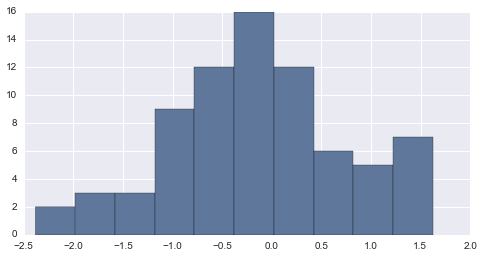
\includegraphics[width=0.8\textwidth]{test_resolution.png}
  \caption{Processing time per frame at various resolutions.}
\end{figure}

\begin{figure}[H]
  \centering
    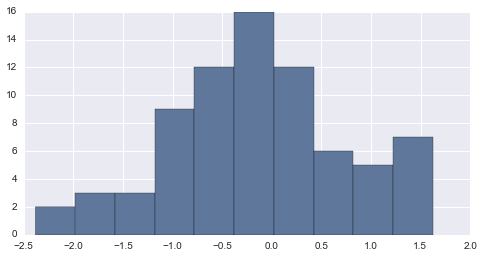
\includegraphics[width=0.8\textwidth]{test_flow.png}
  \caption{Processing time per frame for various magnitudes of motion.}
\end{figure}

\section{Conclusion}

\end{document}
